\documentclass[border=4pt]{standalone}
\usepackage{amsmath,amssymb,amsfonts}
\usepackage{xcolor,colortbl,array,booktabs,multirow}
\usepackage{tikz}
\usepackage{pgfplots}
\pgfplotsset{compat=1.16}
\usetikzlibrary{arrows, automata, backgrounds, calendar, chains, decorations,
    matrix, mindmap, patterns, petri, positioning, shadows, shapes.geometric,
    trees, shapes, decorations.pathreplacing, calc, tikzmark, arrows.meta,
    intersections, fit, graphs, quotes, angles, decorations.markings}
\newcommand{\st}{\text{ s.t. }}
\newcommand{\x}{\mathbf{x}}
\renewcommand{\b}{\mathbf{b}}
\renewcommand{\c}{\mathbf{c}}
\newcommand{\A}{\mathbf{A}}
\newcommand{\y}{\mathbf{y}}
\newcommand{\z}{\mathbf{z}}
\newcommand{\R}{\mathbb{R}}
\newcommand{\RR}{\mathbb{R}}
\newcommand{\Z}{\mathbb{Z}}
\newcommand{\ZZ}{\mathbb{Z}}
\newcommand{\npcomplete}{NP-complete}
\providecommand{\true}{\text{TRUE}}
\providecommand{\false}{\text{FALSE}}
\tikzset{vertex/.style={circle,fill=black!25,minimum size=20pt,inner sep=0pt},
    edge/.style={draw,thick,-},weight/.style={font=\small},
    selected vertex/.style={vertex, fill=red!24},
    selected edge/.style={draw,line width=2pt,-,red!50},
    ignored edge/.style={draw,line width=2pt,-,black!20}}
\newcommand{\vect}{\vec}
\providecommand{\ds}{\displaystyle}
\providecommand{\longvect}{\overrightarrow}
\usepackage[normalem]{ulem}
\definecolor{ocre}{RGB}{243,102,25}
\providecommand{\leftB}{\left[}
\providecommand{\rightB}{\right]}
\tikzset{directed/.style={postaction={decorate,decoration={markings,mark=at position .65 with {\arrow{>}}}}},
    directed1/.style={postaction={decorate,decoration={markings,mark=at position .65 with {\arrow{>}}}}}}
\begin{document}
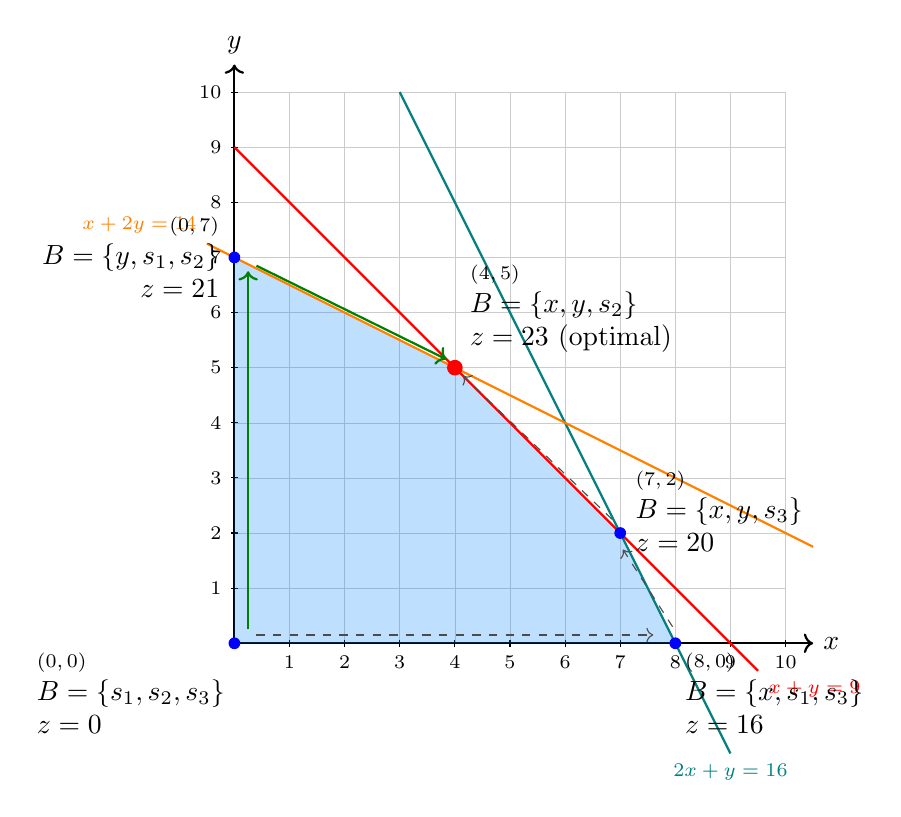
\begin{tikzpicture}[scale=0.7]
    % Grid and axes
    \draw[gray!40, very thin, step=1] (0,0) grid (10,10);
    \draw[->, thick] (0,0) -- (10.5,0) node[right] {$x$};
    \draw[->, thick] (0,0) -- (0,10.5) node[above] {$y$};
    \foreach \x in {1,...,10} \draw (\x,0.06) -- (\x,-0.06) node[below] {\scriptsize \x};
    \foreach \y in {1,...,10} \draw (0.06,\y) -- (-0.06,\y) node[left] {\scriptsize \y};

    % Feasible region
    \fill[blue!50!cyan, opacity=0.25]
        (0,0) -- (8,0) -- (7,2) -- (4,5) -- (0,7) -- cycle;

    % Constraint boundaries
    \draw[red,    thick] (0,9)    -- (9.5,-0.5) node[below right] {\scriptsize $x+y=9$};
    \draw[teal,   thick] (3,10)   -- (9,-2)     node[below]       {\scriptsize $2x+y=16$};
    \draw[orange, thick] (-0.5,7.25) node[above left] {\scriptsize $x+2y=14$}
                                                -- (10.5,1.75);

    % Vertices with basis annotations (one short label per vertex; the basis B
    % and current objective value z are listed in a stacked node beside each).
    \node[fill=blue,circle,inner sep=1.5pt] at (0,0) {};
    \node[below left, align=left] at (0,0)
        {\scriptsize $(0,0)$ \\ $B=\{s_1,s_2,s_3\}$ \\ $z=0$};

    \node[fill=blue,circle,inner sep=1.5pt] at (8,0) {};
    \node[below right, align=left] at (8,0)
        {\scriptsize $(8,0)$ \\ $B=\{x,s_1,s_3\}$ \\ $z=16$};

    \node[fill=blue,circle,inner sep=1.5pt] at (7,2) {};
    \node[right, align=left] at (7.1,2.4)
        {\scriptsize $(7,2)$ \\ $B=\{x,y,s_3\}$ \\ $z=20$};

    \node[fill=red, circle,inner sep=2pt] at (4,5) {};
    \node[above right, align=left] at (4.1,5.1)
        {\scriptsize $(4,5)$ \\ $B=\{x,y,s_2\}$ \\ $z=23$ (optimal)};

    \node[fill=blue,circle,inner sep=1.5pt] at (0,7) {};
    \node[left, align=right] at (-0.1,7)
        {\scriptsize $(0,7)$ \\ $B=\{y,s_1,s_2\}$ \\ $z=21$};

    % Pivot arrows along edges (one possible path: (0,0)->(0,7)->(4,5),
    % an alternate path: (0,0)->(8,0)->(7,2)->(4,5)).
    \draw[->, thick, green!50!black] (0.25,0.25)  -- (0.25,6.75);
    \draw[->, thick, green!50!black] (0.4,6.85)   -- (3.85,5.15);
    \draw[->, dashed, gray!60!black] (0.4,0.15)   -- (7.6,0.15);
    \draw[->, dashed, gray!60!black] (7.95,0.3)   -- (7.05,1.7);
    \draw[->, dashed, gray!60!black] (6.85,2.25)  -- (4.15,4.85);
\end{tikzpicture}
\end{document}
